\documentclass[9pt,aspectratio=169,xcolor=table]{beamer}

%~~~~~~~~~~~~~~~~~~~~~~~~~~~~~~~~~~~~~~~~~~~~~~~~~~~~~~~~~~~~~~~~~~~~~~~~~~~~~~
% Use roboto Font (recommended)
\usepackage[sfdefault]{roboto}
\usepackage[utf8]{inputenc}
\usepackage[T1]{fontenc}
%~~~~~~~~~~~~~~~~~~~~~~~~~~~~~~~~~~~~~~~~~~~~~~~~~~~~~~~~~~~~~~~~~~~~~~~~~~~~~~

%~~~~~~~~~~~~~~~~~~~~~~~~~~~~~~~~~~~~~~~~~~~~~~~~~~~~~~~~~~~~~~~~~~~~~~~~~~~~~~
% Define where theme files are located. ('/styles')
\usepackage{styles/fluxmacros}
\usefolder{styles}
% Use Flux theme v0.1 beta
% Available style: asphalt, blue, red, green, gray
\usetheme[style=hunter]{flux}
%~~~~~~~~~~~~~~~~~~~~~~~~~~~~~~~~~~~~~~~~~~~~~~~~~~~~~~~~~~~~~~~~~~~~~~~~~~~~~~

%~~~~~~~~~~~~~~~~~~~~~~~~~~~~~~~~~~~~~~~~~~~~~~~~~~~~~~~~~~~~~~~~~~~~~~~~~~~~~~
% Extra packages
\usepackage{booktabs}
\usepackage{colortbl}
\usepackage{ragged2e}
\usepackage{amssymb}
\usepackage{multirow}
\usepackage{tikz}
\usetikzlibrary{arrows.meta, positioning, fit, backgrounds, calc, decorations.pathreplacing}
\setbeamertemplate{itemize items}[square]
\usepackage[scaled=.8]{beramono}
\usepackage{listings}
\usepackage{styles/lstlangarm}
\usepackage{array}
\definecolor{bgcolor}{HTML}{F2E9E9}
% lstlangarm.sty references \color{mauve} for string literals but never defines
% it -- only fires when a listing contains a string. Define it here.
\definecolor{mauve}{rgb}{0.58,0,0.82}
% lstlangarm's C style sets commentstyle=green!20, which is unreadable on the
% pink listing background. Darken it globally.
\lstset{commentstyle=\color{green!45!black}}
% ragged-right fixed-width column -- must be defined in the preamble, never
% inside a frame (\newcolumntype's #1 breaks beamer's frame scanner)
\newcolumntype{R}[1]{>{\RaggedRight\arraybackslash}p{#1}}
%~~~~~~~~~~~~~~~~~~~~~~~~~~~~~~~~~~~~~~~~~~~~~~~~~~~~~~~~~~~~~~~~~~~~~~~~~~~~~~
% Table striping: odd rows white, even rows very light gray.
% Needs \documentclass[...,xcolor=table]{beamer} (beamer loads xcolor itself,
% so the option must go on the class, not \usepackage).
\definecolor{stripe}{gray}{0.94}
% \striped makes body rows alternate white, gray, white, ... starting white.
% \rowcolors counts from the first coloured body row; the header is not counted.
\newcommand{\striped}{\rowcolors{1}{white}{stripe}}
%~~~~~~~~~~~~~~~~~~~~~~~~~~~~~~~~~~~~~~~~~~~~~~~~~~~~~~~~~~~~~~~~~~~~~~~~~~~~~~

%~~~~~~~~~~~~~~~~~~~~~~~~~~~~~~~~~~~~~~~~~~~~~~~~~~~~~~~~~~~~~~~~~~~~~~~~~~~~~~
% TikZ block styles -- matches ch1/ch2
% Colour variables are named identically in the book's stm32primer.tex, so any
% tikzpicture using only the \tikzset{...} styles below can be copied verbatim
% between slides and book. Only the \definecolor/\colorlet VALUES differ: the
% book is printed, so it keeps every stroke pure black with muted fills. These
% slides are projected, so both fill AND stroke are bright and saturated to
% grab attention -- see stm32primer.tex for the print palette.
\definecolor{blkfill}{HTML}{DDEEDD}
\definecolor{blkline}{HTML}{355E3B}
\definecolor{accentfill}{HTML}{FFE0B2}
\definecolor{accentline}{HTML}{E65100}
\definecolor{memfill}{HTML}{DFF5DA}
\definecolor{memline}{HTML}{2E7D32}
\definecolor{cellfill}{HTML}{FFFFFF}
\definecolor{cellline}{HTML}{424242}
\definecolor{bitmaskfill}{HTML}{DCEBFF}
\definecolor{bitmaskline}{HTML}{1565C0}
\definecolor{bithitfill}{HTML}{FFE0B2}
\definecolor{bithitline}{HTML}{E65100}
\tikzset{
  blk/.style   = {rectangle, rounded corners=2pt, draw=blkline, fill=blkfill,
                  thick, align=center, font=\small, minimum height=9mm, inner sep=3pt},
  cpublk/.style= {rectangle, rounded corners=2pt, draw=accentline, fill=accentfill,
                  thick, align=center, font=\small\bfseries, minimum height=9mm, inner sep=3pt},
  memblk/.style= {rectangle, rounded corners=2pt, draw=memline, fill=memfill,
                  thick, align=center, font=\small, minimum height=9mm, inner sep=3pt},
  cell/.style  = {rectangle, draw=cellline, fill=cellfill, align=center,
                  font=\small\ttfamily, minimum height=7mm, inner sep=2pt},
  bitcell/.style={rectangle, draw=cellline, fill=cellfill, thick,
                  minimum width=5.4mm, minimum height=5.4mm, inner sep=0pt,
                  font=\scriptsize\ttfamily, anchor=center},
  bitmask/.style={bitcell, fill=bitmaskfill, draw=bitmaskline},
  bithit/.style ={bitcell, fill=bithitfill, draw=bithitline, font=\scriptsize\ttfamily\bfseries},
  rowlab/.style ={font=\scriptsize, text=Gray, anchor=east},
  oplab/.style  ={font=\scriptsize\itshape, text=Gray, anchor=west},
  lbl/.style   = {font=\scriptsize, text=Gray},
  flow/.style  = {-{Stealth[length=2mm]}, thick, draw=blkline},
  busline/.style={thick, draw=cellline},
}
% NOTE (theme quirks -- all fail SILENTLY, always page through the PDF):
%  - a second \\ inside a nested {...} group in a TikZ node breaks parsing
%  - {\small ...} wrapped around a nested itemize eats the frame title + list
%  - \usebeamercolor on a [plain] frame falls through to an unstyled default
%  - \newcolumntype inside a frame breaks beamer's frame scanner
%  - lstlisting needs \begin{frame}[fragile]
%  - a TikZ picture wider than its column silently overflows into neighbours
%~~~~~~~~~~~~~~~~~~~~~~~~~~~~~~~~~~~~~~~~~~~~~~~~~~~~~~~~~~~~~~~~~~~~~~~~~~~~~~

%%%%%%%%%%%%%%%%%%%%%%%%%%%%%%%%%%%
%% BEGIN CONDITIONAL COMPILATION %%
%%%%%%%%%%%%%%%%%%%%%%%%%%%%%%%%%%%
\newif\ifwebex
%\webextrue % uncomment to generate section separator
\ifwebex
\AtBeginSection[]{
  \begin{frame}
  \vfill
  \centering
  \begin{beamercolorbox}[sep=8pt,center,shadow=true,rounded=true]{title}
    \usebeamerfont{title}\insertsectionhead\par%
  \end{beamercolorbox}
  \vfill
  \end{frame}
}
\else
\AtBeginSection[]
{
{
    \setbeamercolor{background canvas}{bg=yellow!10}
    \begin{frame}[plain]
        \frametitle{Table of Contents}
        \tableofcontents[currentsection]
    \end{frame}
}
}
\fi
%%%%%%%%%%%%%%%%%%%%%%%%%%%%%%%%%%%
%% END CONDITIONAL COMPILATION   %%
%%%%%%%%%%%%%%%%%%%%%%%%%%%%%%%%%%%

%~~~~~~~~~~~~~~~~~~~~~~~~~~~~~~~~~~~~~~~~~~~~~~~~~~~~~~~~~~~~~~~~~~~~~~~~~~~~~~
% Information
\title{Latches and Flip-Flops}
\subtitle{\emph{Contemporary Digital Electronic Systems} --- Chapter 10}
\author{Mun\'{i}m Zabidi}
\institute{\color{primary}Faculty of Electrical Engineering, Universiti Teknologi Malaysia}
\date{\today}
\titlegraphic{assets/logoutmwhite.png}
\graphicspath{{.}{assets/}}
%~~~~~~~~~~~~~~~~~~~~~~~~~~~~~~~~~~~~~~~~~~~~~~~~~~~~~~~~~~~~~~~~~~~~~~~~~~~~~~

\newcommand{\figh}[2]{\includegraphics[height=#1\textheight]{#2}}

\begin{document}

\titlepage

%===============================================================================
\section{Why This Chapter}
%===============================================================================

\begin{frame}{Why This Chapter Matters}
  \begin{columns}[c]
  \begin{column}{.47\textwidth}
    Every circuit so far was combinational: output $= f$(current input). Counters, state machines and processors must \alert{remember} the past. This chapter adds a \alert{memory element} (latch or flip-flop) and a \alert{clock} that decides when memory may change.
  \end{column}
  \begin{column}{.51\textwidth}
    \begin{block}{After this chapter, you can:}
    {\small
    \begin{enumerate}\itemsep2pt
      \item State how combinational and sequential circuits differ.
      \item Build an SR latch from cross-coupled NAND or NOR gates and analyse it.
      \item Distinguish level-sensitive latches from edge-triggered flip-flops.
      \item Draw the characteristic table, equation and timing of D, SR, JK and T devices.
      \item State setup and hold requirements and find the maximum clock frequency.
    \end{enumerate}}
    \end{block}
  \end{column}
  \end{columns}
\end{frame}

\begin{frame}{An Opening Question}
  \leavevmode\vspace{4mm}
  \begin{center}
  \fbox{\parbox{.78\textwidth}{\centering\vspace{2mm}
  \large For how long before and after the active clock edge must a flip-flop's data stay still? And what limits how fast you may run the clock?
  \vspace{2mm}}}
  \end{center}
  \vspace{4mm}
  We answer both with setup and hold times and the maximum clock frequency.
\end{frame}

\begin{frame}{Sequential Circuit = Logic + State}
  \begin{itemize}\small\itemsep3pt
    \item A sequential circuit is combinational logic plus a bank of flip-flops that store the \alert{state}.
    \item On each active clock edge the flip-flops sample their inputs and update the state. Between edges, the logic computes the next state and the outputs.
  \end{itemize}
  \centering\small\striped
  \begin{tabular}{@{}lR{.2\textwidth}R{.27\textwidth}R{.27\textwidth}@{}}
    \toprule
    & \textbf{Combinational} & \textbf{Latch} & \textbf{Flip-flop} \\
    \midrule
    Depends on & Current input only & Current input (when enabled) and stored value & Stored value, sampled at the clock edge \\
    Stores? & No & Yes, while enable is active & Yes, until the next active edge \\
    Responds to & Any input change (after $t_{pd}$) & Input change \emph{while} enable is high (level-sensitive) & Input value \emph{at} the active edge (edge-triggered) \\
    \bottomrule
  \end{tabular}
\end{frame}

%===============================================================================
\section{Clocks}
%===============================================================================

\begin{frame}{Synchronous and Asynchronous Circuits}
  \centering
  \figh{.28}{seqcir-async}\hspace{10mm}\figh{.28}{seqcir-sync}\\[1mm]
  {\small Asynchronous \hspace{.28\textwidth} Synchronous}
  \begin{itemize}\small\itemsep3pt
    \item \alert{Synchronous}: a clock coordinates all actions: precise timing, reliable, easy to use. Costs clock-distribution power; speed is limited by the slowest path.
    \item \alert{Asynchronous}: responds to input changes without a clock; less predictable.
  \end{itemize}
\end{frame}

\begin{frame}{Clock Signals}
  \begin{columns}[c]
  \begin{column}{.52\textwidth}
    \centering
    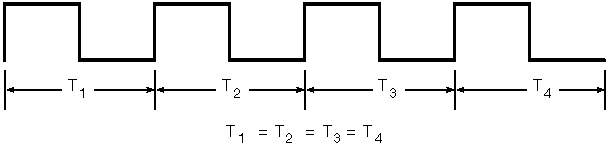
\includegraphics[width=\textwidth]{clock_yes}\\[-1mm]
    {\scriptsize A clock signal}\\[3mm]
    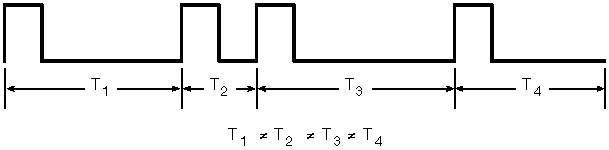
\includegraphics[width=\textwidth]{clock_no}\\[-1mm]
    {\scriptsize Not a clock signal}\\[3mm]
    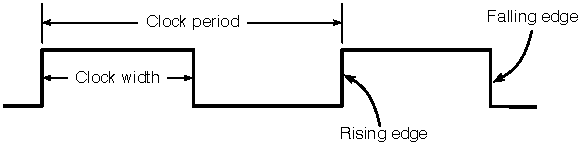
\includegraphics[width=\textwidth]{clock_parts}\\[-1mm]
    {\scriptsize Parts of a clock signal}
  \end{column}
  \begin{column}{.46\textwidth}
    \begin{itemize}\small\itemsep4pt
      \item A clock is a regular pulse train, measured in Hz (GHz in modern circuits).
      \item Most circuits are edge-triggered: \alert{positive-edge} (low-to-high) or \alert{negative-edge} (high-to-low).
      \item \alert{Latches} are level-triggered; \alert{flip-flops} are edge-triggered.
    \end{itemize}
  \end{column}
  \end{columns}
\end{frame}

%===============================================================================
\section{Latches}
%===============================================================================

\begin{frame}{Bistable Circuit}
  \centering
  \figh{.12}{cascadedinverters}
  \begin{itemize}\small\itemsep3pt
    \item Two inverters in a loop have two stable states, so they remember a bit (the basis of SRAM).
    \item The state is random at power-up and cannot be set. Replace the inverters with control gates (NOR) to set and reset it.
  \end{itemize}
\end{frame}

\begin{frame}{SR Latch (NOR)}
  \begin{columns}[c]
  \begin{column}{.4\textwidth}
    \centering
    \figh{.2}{nors_cascaded}\hspace{2mm}\figh{.2}{srlatch}\\[2mm]
    \figh{.18}{srlatchsym}
  \end{column}
  \begin{column}{.58\textwidth}
    \begin{itemize}\small\itemsep3pt
      \item $S = 1, R = 0$: $Q = 1$ (set). $S = 0, R = 1$: $Q = 0$ (reset). $S = R = 0$: hold.
      \item $S = R = 1$: both outputs low (forbidden). Releasing both together gives an unpredictable $Q$: avoid.
    \end{itemize}
    \centering\scriptsize\striped
    \begin{tabular}{@{}cc|cc|l@{}}
      \toprule
      $S$ & $R$ & $Q^+$ & $\overline{Q^+}$ & Action \\
      \midrule
      0&0&$Q$&$\overline{Q}$ & No change \\ 0&1&0&1 & Reset \\ 1&0&1&0 & Set \\ 1&1&0&0 & Forbidden \\
      \bottomrule
    \end{tabular}
  \end{column}
  \end{columns}
\end{frame}

\begin{frame}{SR Latch: Characteristic Table and Timing}
  \begin{columns}[c]
  \begin{column}{.45\textwidth}
    \centering\scriptsize\striped
    \begin{tabular}{@{}cc|cc|cc@{}}
      \toprule
      $S$ & $R$ & $Q$ & $\overline{Q}$ & $Q^+$ & $\overline{Q^+}$ \\
      \midrule
      0&0&0&1&0&1 \\ 0&0&1&0&1&0 \\ 0&1&0&1&0&1 \\ 0&1&1&0&0&1 \\
      1&0&0&1&1&0 \\ 1&0&1&0&1&0 \\ 1&1&0&1&0&0 \\ 1&1&1&0&0&0 \\
      \bottomrule
    \end{tabular}\\[2mm]
    {\small $Q$ = present state; $Q^+$ = next state.}
  \end{column}
  \begin{column}{.53\textwidth}
    \centering
    \figh{.3}{srlatchtiming}
    \begin{itemize}\small
      \item $\overline{Q}$ is the opposite of $Q$ except when $S = R = 1$.
    \end{itemize}
  \end{column}
  \end{columns}
\end{frame}

\begin{frame}{$\overline{S}\,\overline{R}$ Latch (NAND)}
  \begin{columns}[c]
  \begin{column}{.4\textwidth}
    \centering
    \figh{.22}{sr_xcouple}\hspace{2mm}\figh{.18}{srnandlatchsym}
  \end{column}
  \begin{column}{.58\textwidth}
    \centering\small\striped
    \begin{tabular}{@{}cc|cc|l@{}}
      \toprule
      $\overline{S}$ & $\overline{R}$ & $Q^+$ & $\overline{Q^+}$ & Action \\
      \midrule
      0&0&1&1 & Forbidden \\ 0&1&1&0 & Set \\ 1&0&0&1 & Reset \\ 1&1&$Q$&$\overline{Q}$ & No change \\
      \bottomrule
    \end{tabular}
    \begin{itemize}\small\itemsep3pt
      \item Set and reset are \alert{active low}.
      \item More widely used than the NOR latch: NAND gates are usually faster.
    \end{itemize}
  \end{column}
  \end{columns}
\end{frame}

\begin{frame}{Gated SR Latch}
  \begin{columns}[c]
  \begin{column}{.5\textwidth}
    \centering
    \figh{.2}{gatedsrnorlatch}\hspace{2mm}\figh{.2}{gatedsrnandlatch}\\[1mm]
    {\scriptsize NOR-based \hspace{.15\textwidth} NAND-based}\\[2mm]
    \figh{.18}{gatedsrlatchsym}
  \end{column}
  \begin{column}{.48\textwidth}
    \begin{itemize}\small\itemsep3pt
      \item An enable ($EN$) controls a gate in front of $S$ and $R$. With $EN = 0$ the latch holds, whatever $S$ and $R$ do.
      \item With $EN = 1$ the inputs act as in the plain SR latch. Do not apply $S = R = 1$.
    \end{itemize}
    \centering\scriptsize\striped
    \begin{tabular}{@{}c|cc|c|l@{}}
      \toprule
      $EN$ & $S$ & $R$ & $Q^+$ & Action \\
      \midrule
      0&X&X&$Q$ & No change \\ 1&0&0&$Q$ & No change \\ 1&0&1&0 & Reset \\ 1&1&0&1 & Set \\ 1&1&1&X & Forbidden \\
      \bottomrule
    \end{tabular}
  \end{column}
  \end{columns}
\end{frame}

\begin{frame}{Gated SR Latch: Timing}
  \centering
  \figh{.4}{gatedsrlatchtiming}
  \begin{itemize}\small
    \item Output changes only while $EN$ is high.
    \item Both inputs high just before $EN$ falls leaves the latch in a forbidden state.
  \end{itemize}
\end{frame}

\begin{frame}{D Latch}
  \begin{columns}[c]
  \begin{column}{.55\textwidth}
    \centering
    \figh{.17}{dlatch5gate}\hspace{2mm}\figh{.17}{dlatch4gate}\\[1mm]
    {\scriptsize Gated SR latch plus an inverter \hspace{.05\textwidth} Improved version}\\[2mm]
    \figh{.16}{dlatchsym}
  \end{column}
  \begin{column}{.43\textwidth}
    \begin{itemize}\small\itemsep3pt
      \item Inputs: enable $EN$ and data $D$.
      \item $EN = 1$: $Q$ follows $D$ (``transparent''). $EN = 0$: $Q$ holds the value $D$ had when $EN$ fell.
    \end{itemize}
    \centering\scriptsize\striped
    \begin{tabular}{@{}c|c|c|l@{}}
      \toprule
      $EN$ & $D$ & $Q^+$ & Action \\
      \midrule
      0&X&$Q$ & Storage \\ 1&0&0 & Transparent \\ 1&1&1 & Transparent \\
      \bottomrule
    \end{tabular}
  \end{column}
  \end{columns}
\end{frame}

\begin{frame}{D Latch: Timing}
  \centering
  \figh{.35}{dlatchtiming}
  \begin{itemize}\small
    \item While $EN$ is high the output tracks $D$; when $EN$ falls the output freezes.
  \end{itemize}
\end{frame}

%===============================================================================
\section{Flip-Flops}
%===============================================================================

\begin{frame}{Edge-Triggered Flip-Flops}
  \begin{columns}[c]
  \begin{column}{.55\textwidth}
    \begin{itemize}\small\itemsep3pt
      \item Flip-flops respond to clock \alert{edges}; latches respond to clock \alert{levels}.
      \item \alert{PET}: rising edge. \alert{NET}: falling edge.
      \item In symbols the clock input is a triangle; a bubble marks negative-edge sensitivity.
    \end{itemize}
    \begin{alertblock}{Clock edge $\ne$ clock level}
      \small A flip-flop updates at one instant. A latch is transparent for the whole active level. Confusing them is a common source of design bugs.
    \end{alertblock}
  \end{column}
  \begin{column}{.43\textwidth}
    \centering
    \figh{.2}{latch_pet}\\{\scriptsize PET}\\[2mm]
    \figh{.2}{latch_net}\\{\scriptsize NET}
  \end{column}
  \end{columns}
\end{frame}

\begin{frame}{D Flip-Flop}
  \begin{columns}[c]
  \begin{column}{.4\textwidth}
    \centering
    \figh{.17}{dffsym}\\[2mm]
    \centering\scriptsize\striped
    \begin{tabular}{@{}c|c|c|l@{}}
      \toprule
      $Clk$ & $D$ & $Q^+$ & Action \\
      \midrule
      0&X&$Q$ & No change \\ 1&X&$Q$ & No change \\ $\uparrow$&0&0 & Reset \\ $\uparrow$&1&1 & Set \\
      \bottomrule
    \end{tabular}
  \end{column}
  \begin{column}{.58\textwidth}
    \begin{itemize}\small\itemsep3pt
      \item Stores one bit or delays a signal by one clock cycle.
      \item Unlike the D latch it has \alert{no transparent mode}: it copies $D$ to $Q$ at the clock edge, and $Q$ is then unchanged until the next edge.
    \end{itemize}
    \centering
    \figh{.3}{dlatchnfrenstiming}\hspace{2mm}\figh{.3}{dlatchnfrenscir}
  \end{column}
  \end{columns}
\end{frame}

\begin{frame}{JK Flip-Flop}
  \begin{columns}[c]
  \begin{column}{.4\textwidth}
    \centering
    \figh{.17}{jkff_sym}\\[2mm]
    \scriptsize\striped
    \begin{tabular}{@{}c|cc|c|l@{}}
      \toprule
      $Clk$ & $J$ & $K$ & $Q^+$ & Action \\
      \midrule
      0/1&X&X&$Q$ & No change \\ $\uparrow$&0&0&$Q$ & No change \\ $\uparrow$&0&1&0 & Reset \\ $\uparrow$&1&0&1 & Set \\ $\uparrow$&1&1&$\overline{Q}$ & Toggle \\
      \bottomrule
    \end{tabular}
  \end{column}
  \begin{column}{.58\textwidth}
    \begin{itemize}\small\itemsep3pt
      \item Versatile: set, reset, hold and \alert{toggle}.
      \item It removes the ambiguity of the SR latch: $J = K = 1$ is allowed and toggles.
    \end{itemize}
    \centering
    \figh{.3}{jkfftiming}
  \end{column}
  \end{columns}
\end{frame}

\begin{frame}{T Flip-Flop}
  \begin{columns}[c]
  \begin{column}{.4\textwidth}
    \centering
    \figh{.17}{tffsym}\\[2mm]
    \scriptsize\striped
    \begin{tabular}{@{}c|c|c|l@{}}
      \toprule
      $Clk$ & $T$ & $Q^+$ & Action \\
      \midrule
      0/1&X&$Q$ & No change \\ $\uparrow$&0&$Q$ & Hold \\ $\uparrow$&1&$\overline{Q}$ & Toggle \\
      \bottomrule
    \end{tabular}
  \end{column}
  \begin{column}{.58\textwidth}
    \begin{itemize}\small\itemsep3pt
      \item $T = 0$: the clock has no effect. $T = 1$: the output toggles on each active edge.
    \end{itemize}
    \centering
    \figh{.3}{tfftiming}
  \end{column}
  \end{columns}
\end{frame}

%===============================================================================
\section{Describing Operation}
%===============================================================================

\begin{frame}{Describing a Flip-Flop}
  \begin{itemize}\small\itemsep4pt
    \item The \alert{characteristic table} shows the next state $Q^+$ for each present state and input. Three descriptions follow from it:
    \item \alert{Characteristic equation}: $Q^+$ as a function of $Q$ and the inputs.
    \item \alert{Excitation table}: the inputs needed to cause a desired transition $Q \to Q^+$.
    \item \alert{State diagram}: circles for the two states, arrows for transitions.
  \end{itemize}
  \begin{block}{Characteristic equations}
    \small
    D: $Q^+ = D$ \qquad T: $Q^+ = T \oplus Q$\\
    JK: $Q^+ = J\overline{Q} + \overline{K}Q$ \qquad SR: $Q^+ = S + \overline{R}Q$, with $SR = 0$
  \end{block}
\end{frame}

\begin{frame}{D and T: Excitation Tables and State Diagrams}
  \begin{columns}[t]
  \begin{column}{.5\textwidth}
    \centering\small D flip-flop\\[1mm]
    \scriptsize\striped
    \begin{tabular}{@{}cc|c@{}}
      \toprule
      $Q$ & $Q^+$ & $D$ \\
      \midrule
      0&0&0 \\ 0&1&1 \\ 1&0&0 \\ 1&1&1 \\
      \bottomrule
    \end{tabular}\\[2mm]
    \figh{.18}{stdd}
  \end{column}
  \begin{column}{.5\textwidth}
    \centering\small T flip-flop\\[1mm]
    \scriptsize\striped
    \begin{tabular}{@{}cc|c@{}}
      \toprule
      $Q$ & $Q^+$ & $T$ \\
      \midrule
      0&0&0 \\ 0&1&1 \\ 1&0&1 \\ 1&1&0 \\
      \bottomrule
    \end{tabular}\\[2mm]
    \figh{.18}{stdt}
  \end{column}
  \end{columns}
\end{frame}

\begin{frame}{JK and SR: Excitation Tables and State Diagrams}
  \begin{columns}[t]
  \begin{column}{.5\textwidth}
    \centering\small JK flip-flop\\[1mm]
    \scriptsize\striped
    \begin{tabular}{@{}cc|cc@{}}
      \toprule
      $Q$ & $Q^+$ & $J$ & $K$ \\
      \midrule
      0&0&0&$\times$ \\ 0&1&1&$\times$ \\ 1&0&$\times$&1 \\ 1&1&$\times$&0 \\
      \bottomrule
    \end{tabular}\\[2mm]
    \figh{.18}{stdjk}
  \end{column}
  \begin{column}{.5\textwidth}
    \centering\small SR latch\\[1mm]
    \scriptsize\striped
    \begin{tabular}{@{}cc|cc@{}}
      \toprule
      $Q$ & $Q^+$ & $S$ & $R$ \\
      \midrule
      0&0&0&$\times$ \\ 0&1&1&0 \\ 1&0&0&1 \\ 1&1&$\times$&0 \\
      \bottomrule
    \end{tabular}\\[2mm]
    \figh{.18}{stdsr}
  \end{column}
  \end{columns}
\end{frame}

%===============================================================================
\section{Practical Aspects}
%===============================================================================

\begin{frame}{Setup and Hold Times}
  \centering
  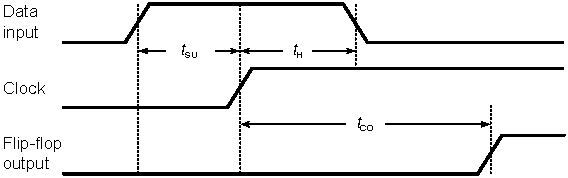
\includegraphics[width=.65\textwidth]{fftiming}
  \begin{itemize}\small\itemsep3pt
    \item \alert{Setup time} $t_{SU}$: the input must be stable this long \emph{before} the clock edge.
    \item \alert{Hold time} $t_H$: the input must stay stable this long \emph{after} the edge.
    \item \alert{Clock-to-output delay} $t_{CO}$: time from the clock edge to a change at the output.
    \item If setup or hold is not met, the flip-flop may not capture the data reliably.
  \end{itemize}
\end{frame}

\begin{frame}{Maximum Clock Frequency}
  \begin{columns}[c]
  \begin{column}{.5\textwidth}
    \[ f_{\max} = \frac{1}{t_{CO} + t_{CPD} + t_{SU}} \]
    \begin{itemize}\small\itemsep3pt
      \item AND, OR and XOR delays: 10, 11 and 16 ns. $t_{CO} = 10$ ns, $t_{SU} = 3$ ns.
      \item Critical path: XOR, then AND, then OR.
    \end{itemize}
    \small
    $t_{CPD} = 16 + 10 + 11 = 37$ ns\\
    $f_{\max} = 1/(10 + 37 + 3)\ \text{ns} = 20$ MHz
  \end{column}
  \begin{column}{.48\textwidth}
    \centering
    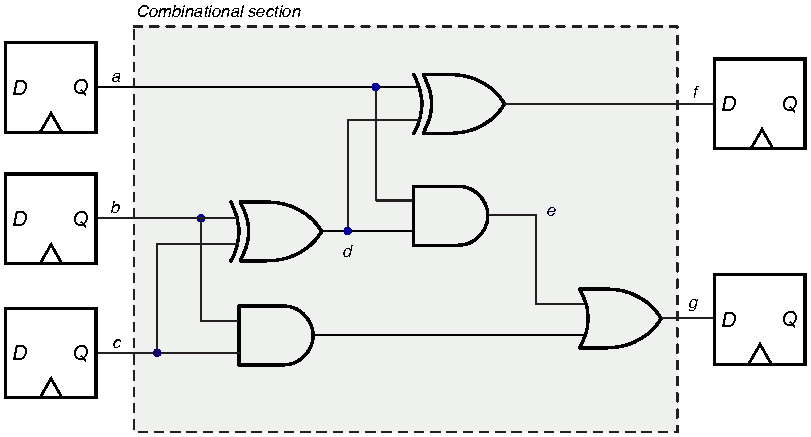
\includegraphics[width=\textwidth]{criticalpath-fx21}
  \end{column}
  \end{columns}
\end{frame}

\begin{frame}{Back to the Opening Question}
  \begin{block}{Setup and hold}
    \small Data must be stable for $t_{SU}$ \emph{before} and $t_H$ \emph{after} every active edge. Inside that window the captured value cannot be relied on.
  \end{block}
  \begin{block}{Limit on the clock}
    \small Between two edges the signal must leave a flip-flop ($t_{CO}$), cross the logic ($t_{CPD}$) and meet setup at the next one ($t_{SU}$): $f_{\max} = 1/(t_{CO} + t_{CPD} + t_{SU})$.
  \end{block}
\end{frame}

\begin{frame}{Flip-Flop Conversion}
  \begin{columns}[c]
  \begin{column}{.5\textwidth}
    \centering
    \figh{.18}{jkff2dff}\hspace{2mm}\figh{.18}{jkff2tff}\\
    {\scriptsize JK to D (inverter between J and K) \hspace{2mm} JK to T (tie J and K)}\\[2mm]
    \figh{.18}{dff2tff}\hspace{2mm}\figh{.18}{dff2jkff}\\
    {\scriptsize D to T ($D = T \oplus Q$) \hspace{4mm} D to JK}
  \end{column}
  \begin{column}{.48\textwidth}
    \begin{itemize}\small\itemsep3pt
      \item The JK flip-flop can be turned into any other type.
      \item A JK flip-flop is not a drop-in replacement for an SR latch: it is edge-triggered, the latch level-sensitive, so substitution changes \emph{when} the circuit reacts.
      \item Modern designs favour D flip-flops; convert a D flip-flop with the target's characteristic equation:
    \end{itemize}
    \small
    T: $Q^+ = T \oplus Q$, so feed $T \oplus Q$ to $D$.\\
    JK: $Q^+ = J\overline{Q} + \overline{K}Q$, so feed that to $D$.
  \end{column}
  \end{columns}
\end{frame}

\begin{frame}{Comparing Flip-Flops}
  \begin{columns}[c]
  \begin{column}{.5\textwidth}
    \centering\small\striped
    \begin{tabular}{@{}cc|cc|c|cc|c@{}}
      \toprule
      $Q$ & $Q^+$ & $S$ & $R$ & $D$ & $J$ & $K$ & $T$ \\
      \midrule
      0&0&0&$\times$&0&0&$\times$&0 \\
      0&1&1&0&1&1&$\times$&1 \\
      1&0&0&1&0&$\times$&1&1 \\
      1&1&$\times$&0&1&$\times$&0&0 \\
      \bottomrule
    \end{tabular}
  \end{column}
  \begin{column}{.48\textwidth}
    \begin{itemize}\small\itemsep3pt
      \item \alert{New designs}: D flip-flops: efficient, easy to design, supported by ASIC/FPGA tools.
      \item \alert{SSI/MSI}: JK: versatile, but more wiring.
      \item \alert{Counters}: T: least logic.
    \end{itemize}
  \end{column}
  \end{columns}
\end{frame}

%===============================================================================
\section{Flip-Flop and Clock ICs}
%===============================================================================

\begin{frame}{74x74 and 74x76}
  \begin{columns}[c]
  \begin{column}{.5\textwidth}
    \centering
    \figh{.25}{74x74}\hspace{4mm}\figh{.25}{74x76}\\[1mm]
    {\scriptsize 74x74: two PET D flip-flops \hspace{.05\textwidth} 74x76: two NET JK flip-flops}
  \end{column}
  \begin{column}{.48\textwidth}
    \begin{itemize}\small\itemsep3pt
      \item Each has asynchronous $\overline{\text{PR}}$ (preset: $Q = 1$) and $\overline{\text{CLR}}$ (clear: $Q = 0$), working regardless of the clock.
      \item With both inactive, the device captures $D$ (or $J$, $K$) on the active edge.
      \item These SSI chips are for labs, but asynchronous preset/clear are still used to initialise circuits.
    \end{itemize}
  \end{column}
  \end{columns}
\end{frame}

\begin{frame}{74x74 Truth Table}
  \centering\small\striped
  \begin{tabular}{@{}ccccc@{}}
    \toprule
    Preset & Clear & $D$ & Clock & $Q^+$ \\
    \midrule
    1&1&0&$\uparrow$&0 \\ 1&1&1&$\uparrow$&1 \\ 1&1&X&0&$Q$ \\ 1&1&X&1&$Q$ \\
    0&1&X&X&1 \\ 1&0&X&X&0 \\ 0&0&X&X&not allowed \\
    \bottomrule
  \end{tabular}
\end{frame}

\begin{frame}{The 555 Timer as a Clock}
  \begin{columns}[c]
  \begin{column}{.45\textwidth}
    \centering
    \figh{.2}{555pinout}\\[2mm]
    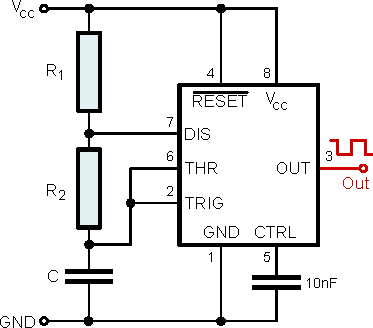
\includegraphics[width=.7\textwidth]{555_astable}
  \end{column}
  \begin{column}{.53\textwidth}
    \begin{itemize}\small\itemsep3pt
      \item A clock has a \alert{frequency} and a \alert{duty cycle} (percent of the period spent high).
      \item In astable mode, $R_1$, $R_2$ and $C$ set the timing:
    \end{itemize}
    \small
    $f = \dfrac{1.44}{(R_1 + 2R_2)C}$, \quad $D = \dfrac{R_1 + R_2}{R_1 + 2R_2}\times 100\%$\\[1mm]
    $t_{high} = 0.693(R_1 + R_2)C$, \quad $t_{low} = 0.693R_2C$
    \begin{itemize}\small
      \item Cheap, but accuracy depends on component tolerance. Use a crystal oscillator when stability matters.
    \end{itemize}
  \end{column}
  \end{columns}
\end{frame}

%===============================================================================
\section{Summary}
%===============================================================================

\begin{frame}{Summary}
  \begin{itemize}\itemsep3pt\small
    \item A \alert{sequential} circuit has state; a combinational circuit does not.
    \item A \alert{latch} is level-sensitive (transparent while enabled). A \alert{flip-flop} is edge-triggered.
    \item SR, JK, D and T differ only in their characteristic equation; one type can always be built from another.
    \item \alert{Setup} and \alert{hold} times define the window around the clock edge in which data must be stable. Violating either may produce an unpredictable output.
    \item $f_{\max}$ follows from $t_{CO} + t_{CPD} + t_{SU} \le T_{clk}$.
  \end{itemize}
  \begin{block}{Looking ahead}
    Chapter 11 wires flip-flops into registers: parallel groups that store and shift multi-bit values.
  \end{block}
\end{frame}

\end{document}
